\documentclass[a4paper]{article}
\usepackage{graphicx}
\usepackage{amsmath, amsfonts, geometry, float, listings, enumerate, multicol}
\usepackage{multicol, float, color, colortbl}
\usepackage{tikz, titlesec, parskip, pgfplots, filecontents}
\usepackage{hyperref}
\usepackage{amsmath}
\usepackage{tikz, titlesec, parskip}
\usepackage{tikz,pgfplots}
\usepackage[americanvoltages,fulldiodes,siunitx]{circuitikz}
\usetikzlibrary{shapes,arrows}
\usepackage{enumitem}
\titleformat*{\subsubsection}{\LARGE\bfseries}
\usepackage{subcaption}
\usepackage{caption}
\titlespacing{\section}{0pt}{10pt}{0pt}
\titlespacing{\subsection}{0pt}{10pt}{0pt}
\titlespacing{\subsubsection}{0pt}{10pt}{0pt}



\usetikzlibrary{calc,patterns,through}
\newcommand{\arcangle}{%
	\mathord{<\mspace{-9mu}\mathrel{)}\mspace{2mu}}%
}

\renewcommand{\baselinestretch}{1.4}
 \geometry{
 a4paper,
 total={170mm,257mm},
 left=20mm,
 top=20mm,
 }
\usepackage{fancyhdr}
\usepackage{indentfirst}
\pagestyle{fancy}
\fancyhf{}
\rhead{\textbf{پردازش تصاویر دیجیتال}}
\lhead{\textbf{تمرین سری ششم}}
\cfoot{(\space \space \space \space \textbf{\thepage}  \space \space \space)}
\renewcommand{\headrulewidth}{1pt}
\renewcommand{\footrulewidth}{1pt}

 
\usepackage{xepersian}
\setlatintextfont{Times New Roman}
\settextfont{XB Niloofar}
\setdigitfont{XB Niloofar}
\DefaultMathsDigits

\makeatletter
\bidi@patchcmd{\@Abjad}{آ}{الف}
{\typeout{Succeeded in changing آ into الف}}
{\typeout{Failed in changing آ into الف}}
\makeatother
\PersianAlphs

\begin{document}
\begin{minipage}{0.6\textwidth}
\begin{bf}
	\begin{center}
		به نام خدا\\
		\vspace{0.25cm}
		دانشگاه صنعتی شریف\\
		\vspace{0.25cm}
		دانشکده مهندسی برق\\
		\vspace{0.5cm}
	
	\large
	دکتر عمادالدین فاطمی‌زاده - پردازش تصاویر دیجیتال \\
	نیم سال دوم
	۱۴۰۱-۱۴۰۰\\
	\Large
	\vspace{0.4cm}
	تمرین عملی سری ششم\\
	\end{center}
\end{bf}
\normalsize
\end{minipage} \hfill
\begin{minipage}{0.35\textwidth}
\begin{flushleft}

\includegraphics[width=0.5\textwidth]{Shariflogo.png}\\ \large
\end{flushleft}

 \end{minipage}
\\

\rule[0.1\baselineskip]{\textwidth}{1pt}

\large
\section*{
لطفاً به نکات زیر توجه بفرمایید: (رعایت نکردن این موارد باعث کاهش نمره می‌شود.)
}

\begin{enumerate}
	\item 
نتایج و پاسخ های خود را در یک فایل با فرمت zip به نام
\LR{HW$6$-Name-StudentNumber}
 در سایت  
\href{https://quera.org/course/add_to_course/course/10598/}{\lr{Quera}} 
 قرار دهید. همچنین فایل پایتون یا متلب خود را به همان نام در قسمت مخصوص به خود آپلود کنید.
\item 
کسب نمره کامل در هر سوال مستلزم تحویل  
\textbf{کدها (40 نمره)}
 و
\textbf{توضیحات (30 نمره)}
و
\textbf{نتایج (30 نمره)}
 می‌باشد. 
\item 
کدهای شما تماماً باید توسط خودتان نوشته شده باشند. هرگونه استفاده از کد دیگران، اعم از دوستان و اینترنت، به هر شکل ممکن، تقلب محسوب می‌شود و نمره تمام تمرینات جاری و تمام تمرینات قبلی صفر خواهد شد. با اجرای این کدها باید همان نتایجی که فرستاده اید قابل بازیابی باشند. برنامه شما باید به گونه‌ای باشد که بدون نیاز به هیچ تغییری قابل اجرا باشد، در غیر این‌ صوررت هیچ نمره‌ای تعلق نخواهد گرفت. 
\item 
برای تمام سؤالات، باید جزئیات روشی که استفاده کرده‌اید را توضیح دهید و نتایجی که گرفته‌اید را ارائه دهید. این توضیحات می‌تواند در یک فایل  pdf  و یا در یک فایل  ipynb باشد. در توضیحات، باید اشاره کامل به کارهایی که انجام داده‌اید بنمایید به طوری که یک شخص آگاه از موارد درس بتواند به آسانی متوجه کاری که شما انجام داده‌اید شود.
\item 
در طول ترم امکان ارسال با تاخیر پاسخ  همه‌ی تمارین تا سقف شش روز و در مجموع بیست و یک روز وجود دارد. پس از گذشت این مدت، پاسخ‌های ارسال‌شده پذیرفته نخواهند بود. همچنین، به ازای هر روز تأخیر غیر مجاز  بیست درصد از نمره تمرین به صورت ساعتی کسر خواهد شد.
\item 
 اگر از
\lr{Jupyter notebook} 
 استفاده می‌کنید، میتوانید خروجی‌ها‌ را پاک کنید تا حجم فایل تحویلی زیاد نشود.
\item 
مهلت تحویل: 
\item 
نام طراح هر سوال در زیر آن نوشته شده است و شما میتوانید سوالات خود را از طریق ایمیل یا تلگرام از طراح سوال بپرسید.
\\
ارسلان فیروزی:
\lr{Arsalan.firoozi@gmail.com } - \lr{@Arsalanfiroozi}
\\
سید سعید رضوی:
\lr{Saeedrazavi890@gmail.com} - \lr{@RazooIs}
\\
امیرحسین جوادی:
\lr{Javadiamirhosein.2000@gmail.com} - \lr{@Amirhosein\_javadi}
\\
امیررضا حاتمی‌پور:
\lr{arhp78@gmail.com} - \lr{@Arhp78}
\end{enumerate}
\rule[0.1\baselineskip]{\textwidth}{1pt}

\clearpage
\section{لاین دیتکشن}
\textbf{طراح :‌ امیرحسین جوادی}
\vspace{0.5cm}
\\
در این تمرین روش هاف 
\lr{(Hough)}
 برای پیدا کردن خطوط در یک تصویر را پیاده سازی می‌نمایید. دقت نمایید که فقط از توابع آماده‌ای که در ادامه گفته می‌شود می‌توانید استفاده کنید و بقیه موارد را خود شما باید پیاده سازی کنید.
\begin{enumerate}
	\item 
دو تصویر
 \lr{im01.jpg}
 و
 \lr{im02.jpg}
	 را در نظر بگیرید. ابتدا لبه‌های این دو تصویر را با روش دلخواه خود به دست آورده و تصاویر آن ها را با نام‌های
	\lr{res01.jpg}
	 و
	\lr{res02.jpg}
	 به ترتیب برای تصاویر اول و دوم ذخیره کنید. برای به دست آوردن لبه‌ها می‌توانید از توابع لبه‌یابی آماده استفاده نمایید
	\begin{figure}[H]
		\centering
		\begin{subfigure}{.49\textwidth}
			\centering
			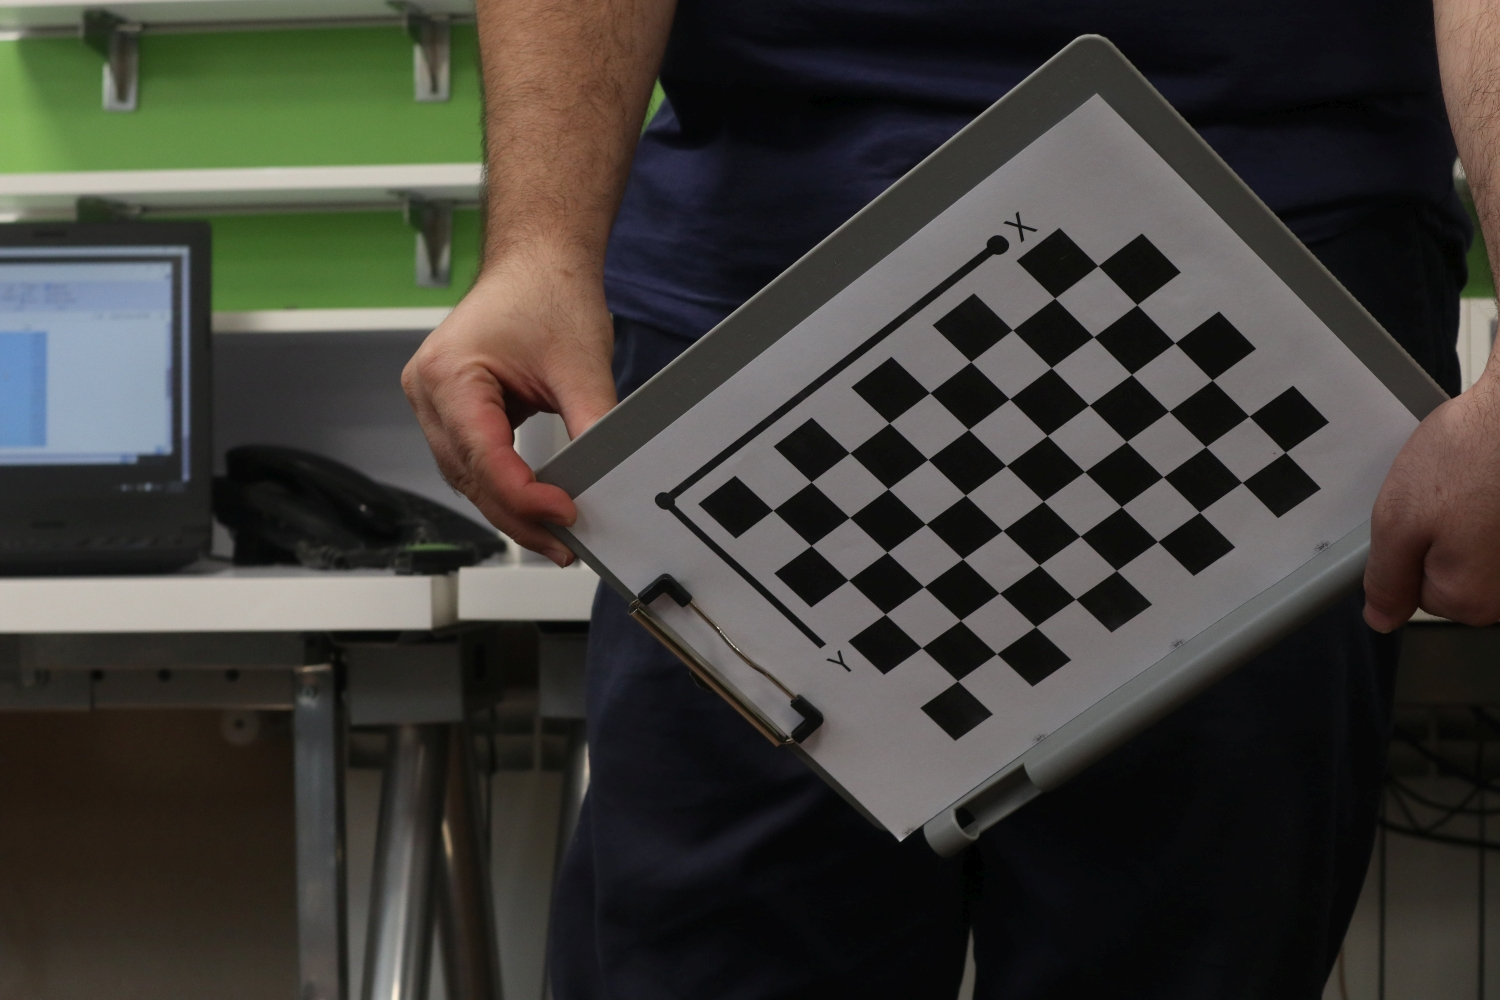
\includegraphics[width=.75\linewidth]{im01}
			\caption{\lr{im01}}
		\end{subfigure}
		\begin{subfigure}{.49\textwidth}
			\centering
			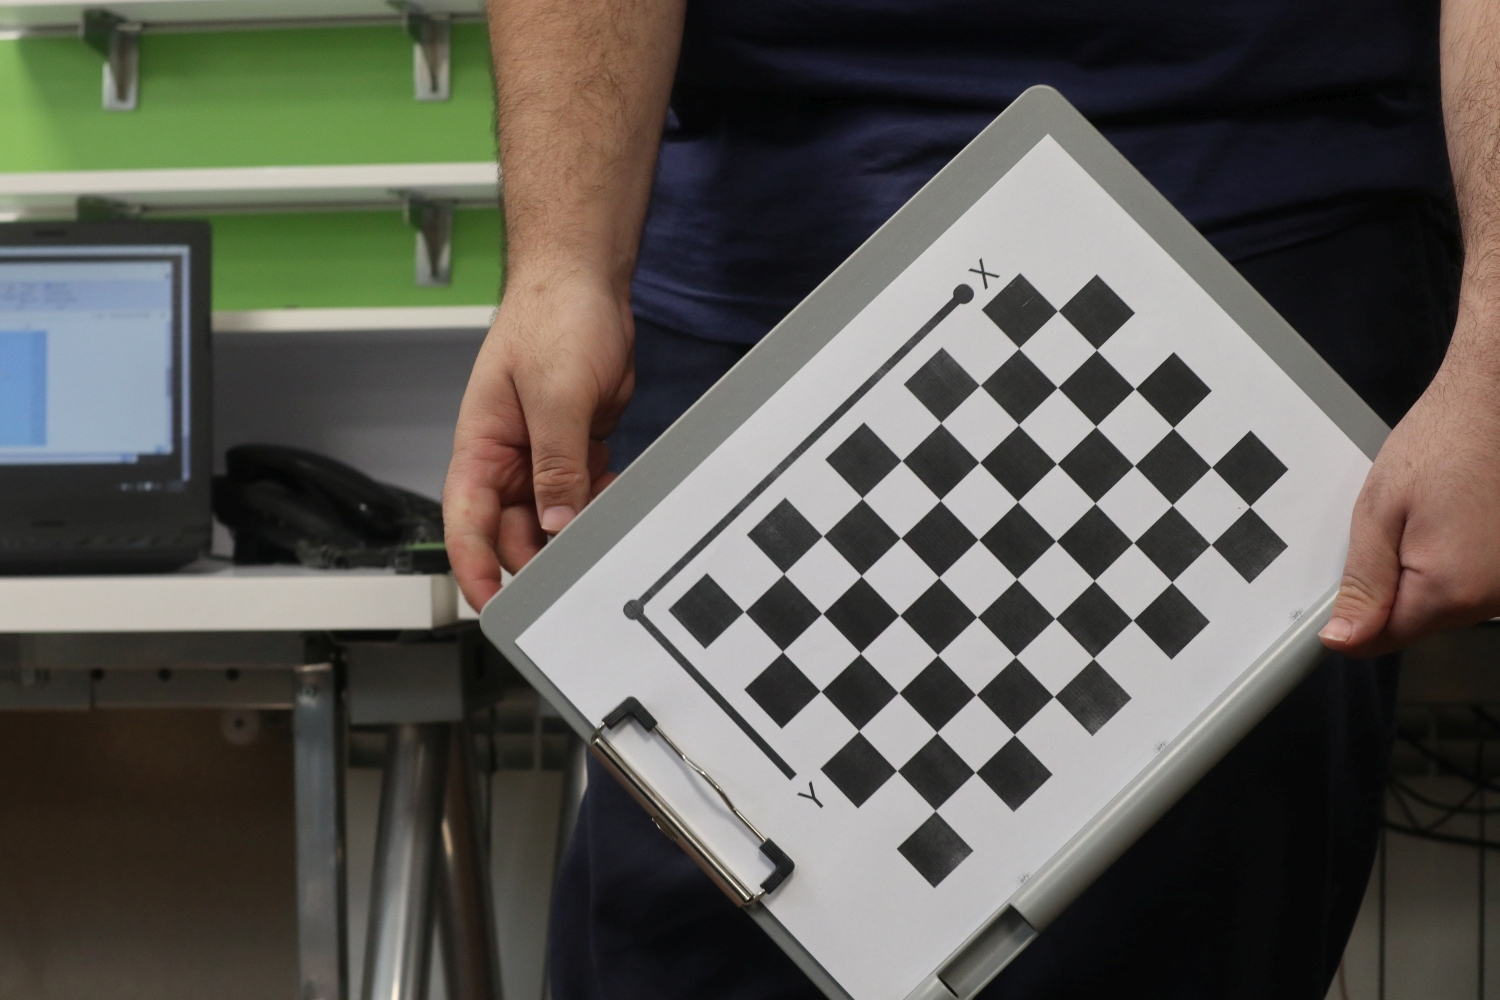
\includegraphics[width=.75\linewidth]{im02}
			\caption{\lr{im02}}
		\end{subfigure}
		\caption{}
	\end{figure}
	\item 
خطوط را در دستگاه قطبی در نظر بگیرید. زاویه خطوط با محور افقی و فاصله آن‌ها تا مبدأ را به دلخواه خود گسسته نمایید و یک ماتریس انباشتی 
	(\lr{accumulator})
برای آن‌ها در نظر بگیرید. تمام درایه‌های این ماتریس را در ابتدا مساوی صفر قرار دهید. برای هر پیکسل لبه، برای تمام خطوطی که از آن پیکسل عبور می‌کنند، درایه متناظر در ماتریس انباشتی را یک واحد افزایش دهید. در انتها، این ماتریس انباشتی را به صورت یک تصویر نمایش داده و با نام 
 \lr{res03-hough-space.jpg}
  و
 \lr{res04-hough-space.jpg}
   به ترتیب برای تصویر اول و دوم ذخیره نمایید. این قسمت را خود شما باید پیاده سازی نمایید و نمی‌توانید از توابع آماده استفاده نمایید.
\begin{figure}[H]
	\centering
	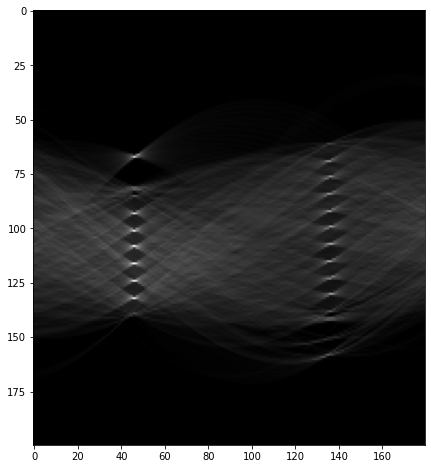
\includegraphics[width=.4\linewidth]{accumulator}
	\caption{\lr{accumulator matrix}}
\end{figure}
\item 
خطوط را از ماتریس‌های انباشتی به دست آورده و روی تصاویر اصلی کشیده و با نام‌های
\lr{res05-lines.jpg}
و
\lr{res06-lines.jpg}
ذخیره نمایید. خطوط را از ماتریس‌های انباشتی طوری به دست بیاورید که تمام خطوط صفحه شطرنجی پیدا شوند. در این صورت تعدادی خطوط دیگر هم در هر تصویر پیدا خواهند شد. با استفاده از دانش پردازش تصویری که دارید، سعی کنید بقیه خطوط را حذف کرده و فقط خطوط محدوده شطرنجی باقی بمانند. خطوط باقی‌مانده را در تصاویر اصلی رسم کرده و با نام‌های
\lr{res07-chess.jpg}
 و
\lr{res08-chess.jpg}
 ذخیره نمایید.
 \item 
از محل طلاقی خطوط محدوده شطرنجی گوشه‌های مربع‌های محدوده شطرنجی را به دست آورده و آن‌ها را روی تصاویر اصلی نشان داده و با نام‌های  
\lr{res09-corners.jpg}
و 
\lr{res10-corners.jpg}
ذخیره نمایید.
\end{enumerate} 
\section{گردالی دیتکشن}
\textbf{طراح :‌ امیرحسین جوادی}
\vspace{0.5cm}
\\
الگوریتم بالا را برای تشخیص دایره استفاده کنید. دقت نمایید که فقط از توابع آماده‌ای که در ادامه گفته می‌شود می‌توانید استفاده کنید و بقیه موارد را خود شما باید پیاده سازی کنید. 
روش 
\lr{Hough transform }
در تمام مسائلی که به فرم 
$ g(v,c) = 0  $ 
که $ v $ بردار مختصات و $ c $ بردار ضرایب باشد، قابل استفاده است. به عنوان مثال، نقاط روی دایره به فرم زیر هستند.
\begin{equation*}
	 (x - c_{1})^{2} + (y - c_{2})^{2} = c_{3}^{2}
\end{equation*}
تفاوت با حالت تشخیص خط این است که در این مسئله سه پارامتر 
$ \{c_{1},c_{2},c_{3}\} $ 
برای مشخص کردن داریم. 
\begin{enumerate}
	\item 
	تصویر
	\lr{im03.jpg}
را در نظر بگیرید. ابتدا لبه‌های این تصویر را با روش دلخواه خود به دست آورده و تصاویر آن را با نام
	\lr{res11.jpg}
ذخیره کنید. برای به دست آوردن لبه‌ها می‌توانید از توابع لبه‌یابی آماده استفاده نمایید. در نهایت با گذاشتن استانه مناسب باید به یک تصویر باینری برسید که لبه را از غیر لبه مشخص کند.
\begin{figure}[H]
	\centering
	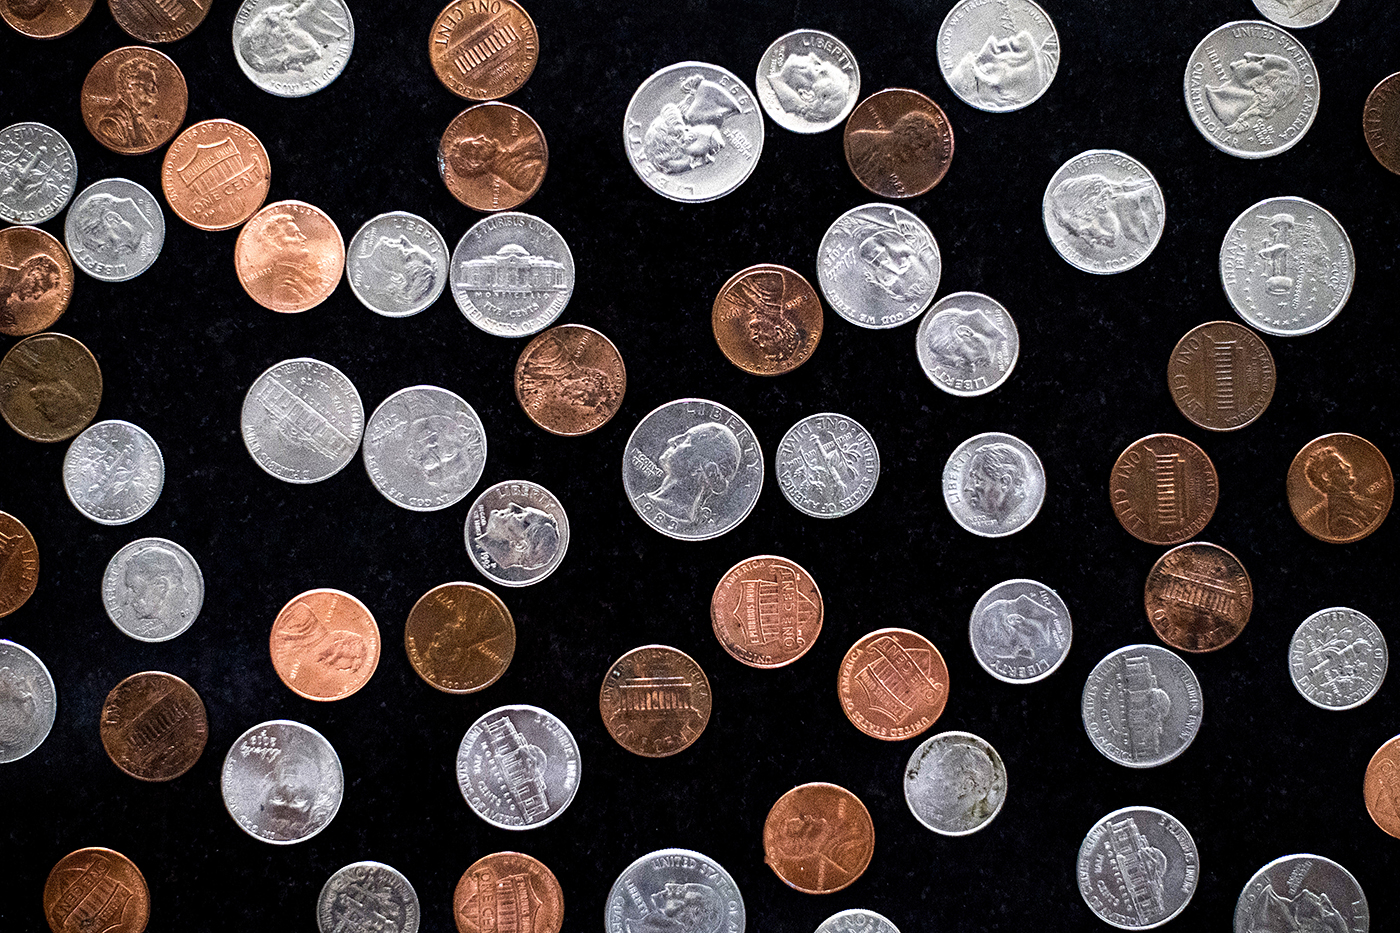
\includegraphics[width=.5\linewidth]{im03}
	\caption{\lr{im03}}
\end{figure}
	\item
	اگر پیکسلی مانند 
	$ (x,y) $
	 روی دایره‌ای به مرکز 
	$ (c_{1},c_{2}) $
	و شعاع 
	$ c_{3} $
	باشد، مکان هندسی نقاط ممکن برای مرکز این دایره برابر است با دایره‌ای به مرکز 
	$ (x,y) $
	و شعاع 
	$ c_{3} $.
اگر برای هر یک از نقاط روی دایره، مکان هندسی ذکر شده را در نظر بگیریم، مشخص است که اشتراک این مکان هندسی‌ها همان مرکز مورد نظر ماست. از این نکته برای پیدا کردن دایره روی تصویر استفاده می‌کنیم. 
به شکل 
\ref{1}
توجه کنید. هدف پیدا کردن مرکز دایره ( نقطه‌ی قرمز) است. همان طور که مشخص است اگر از هر نقطه روی محیط دایره، دایره‌ای به شعاع مورد نظرمان بزنیم از مرکز میگذریم. پس با اشتراک گیری بین این دایره‌ها می‌توانیم به مرکز برسیم.
\begin{figure}[H]
	\centering
	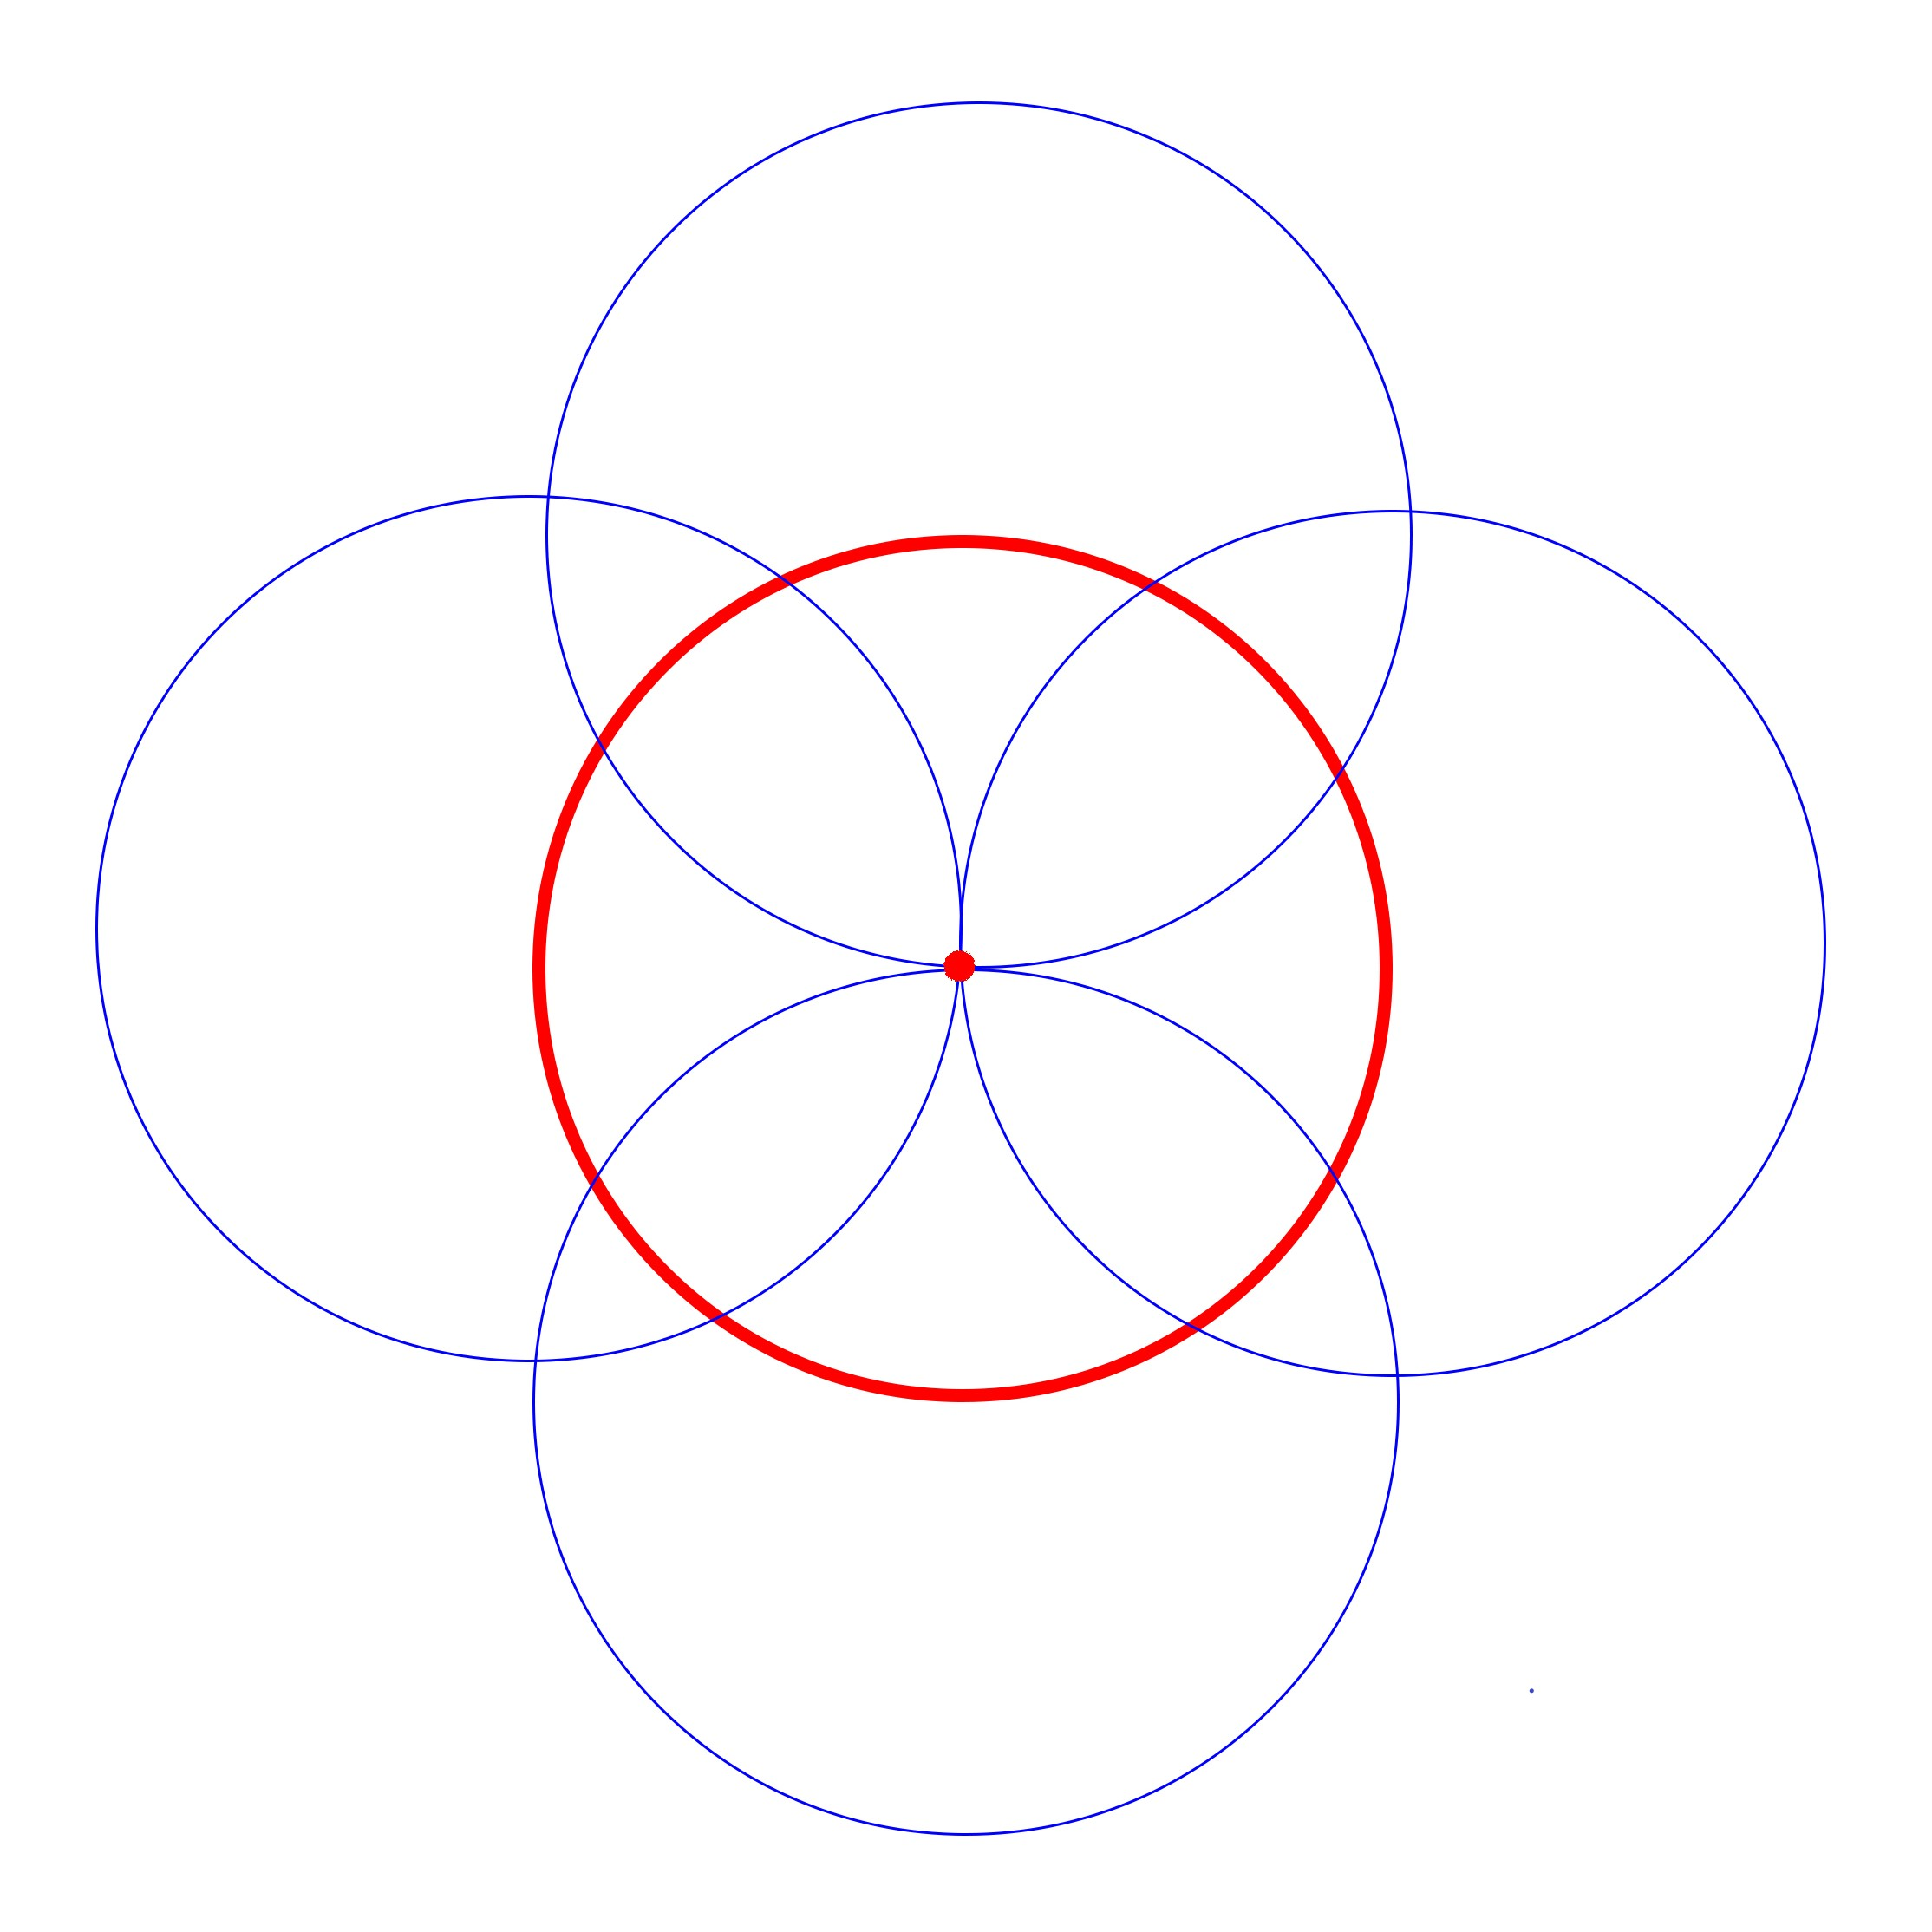
\includegraphics[width=.4\linewidth]{q2}
	\caption{}
	\label{1}
\end{figure}
موردی که وجود دارد این است که ما شعاع را هم به عنوان مجهول داریم. اگر شعاع را داشتیم میتوانستیم به مرکز هر لبه دایره‌ای به شعاع مورد نظر بزنیم و در آخر نقاطی که دایره‌های زیادی از آن‌‌ها گذشته است را به عنوان مراکز احتمالی دایره‌های عکس‌مان گزارش کنیم. حال که شعاع را نداریم باید برای شعاع‌های مختلف این مورد را بررسی کنیم. به همین دلیل است که در این مسئله فضای جست و جو به جا دو بعدی، سه بعدی است و علاوه بر مختصات مرکز، شعاع هم باید جست‌وجو شود.
\\
ماتریس انباشته‌ی سه بعدی به اندازه‌ی 
$ [h,w,c] $
در نظر بگیرید که 
$ [h,w] $
اندازه‌ی تصویر ورودی است و 
$ c $
تعداد شعاع‌هایی است که می‌خواهید بررسی کنید. شعاع‌های مورد نظرتان را می‌توانید به صورت دستی و مخصوص به این مسئله انتخاب کنید. مثلا برای شعاع‌هایی به اندازه‌ی
$ \{50,55,60,65,70 \}$
پیکسل، دایره‌های زیر حداقل در نهایت مشخص می‌شوند. 
\begin{figure}[H]
	\centering
	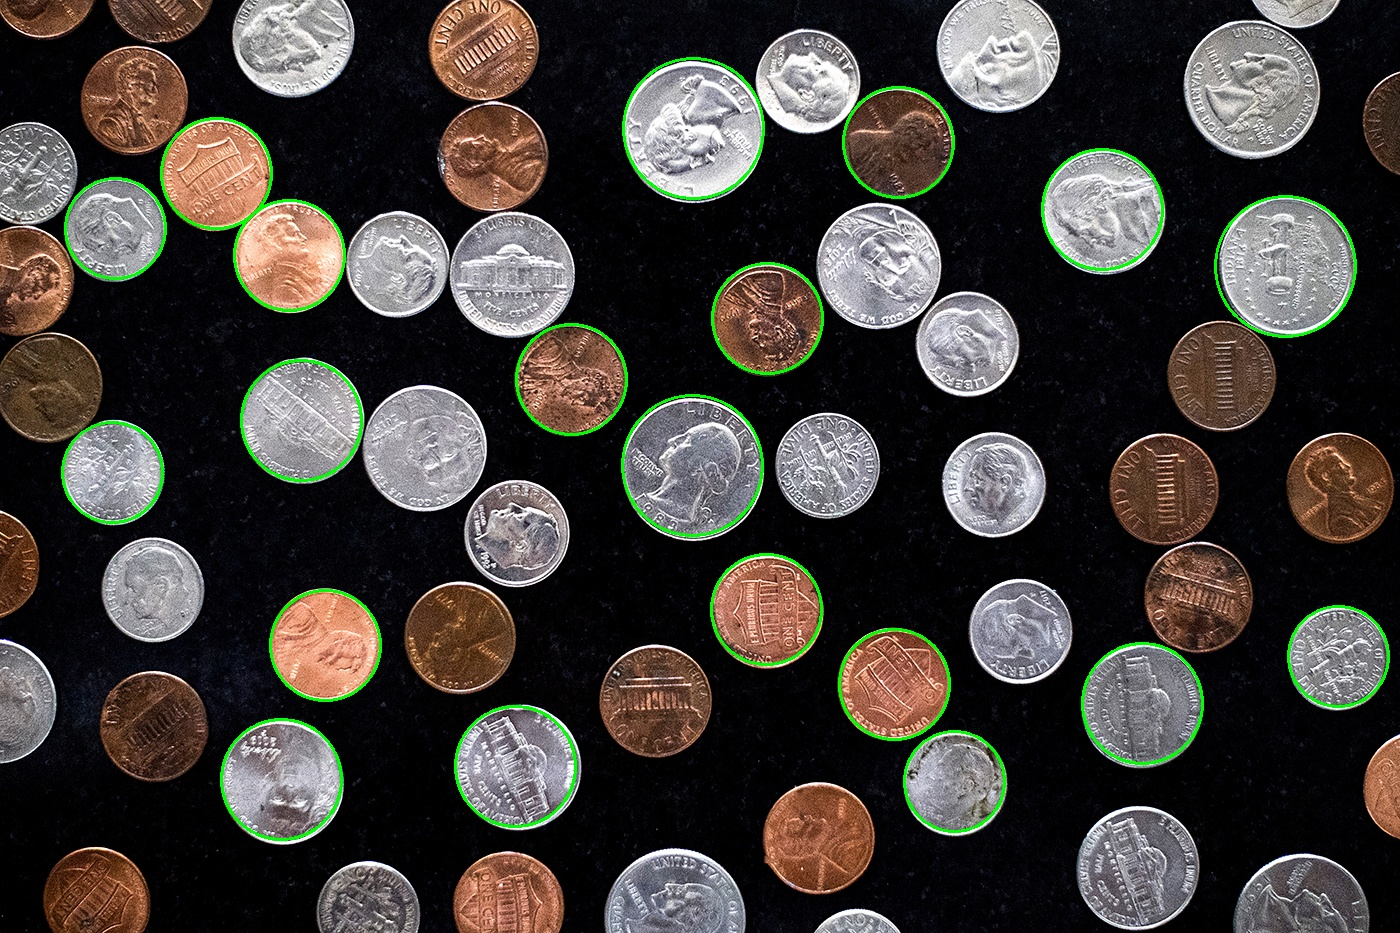
\includegraphics[width=.5\linewidth]{q2_output}
	\caption{}
\end{figure}
بعد از انتخاب شعاع‌های مورد علاقه‌تان برای بررسی این مسئله، ماتریس انباشته متناظر را بسازید. برای هر لایه شعاع متناظر لایه را مشخص کنید. سپس برای هر لبه، دایره‌ای به شعاع مشخص شده بزنید و به درایه‌ی متناظر هر پیکسل روی این دایره در ماتریس انباشته یک واحد اضافه کنید. در نهایت این مرحله شما باید به ماتریس انباشته مورد نظرتان برسید. 
\item 
سپس هر کدام از درایه‌های ماتریس انباشته‌تان که از مقدار
\lr{treshold}
یی بیشتر باشد را میتوانید به عنوان مرکز یک دایره در نظر بگیرید. 
دایره‌ها را از ماتریس انباشتی به دست آورده و روی تصاویر اصلی کشیده و با نام
\lr{res12-circles.jpg}
ذخیره نمایید. همچنین تعداد دایره‌هایی که پیدا کردید را در برنامه چاپ کنید و در گزارشتان بیاورید. نمره‌ نهایی تابع تعداد دایره و دقت   تشخصیص شما (تشخیص حداکثر یک دایره برای هر سکه) است.

\end{enumerate}
\section{\lr{Active Contour}}
\textbf{طراح :‌ ارسلان فیروزی }
\vspace{0.5cm}
\\
در این سوال قصد داریم با استفاده از روش 
\lr{Active Contours}
 سکوی نفتی در عکس 
\lr{im04.jpg}
را تقسیم بندی کنیم. 
\begin{figure}[H]
	\centering
	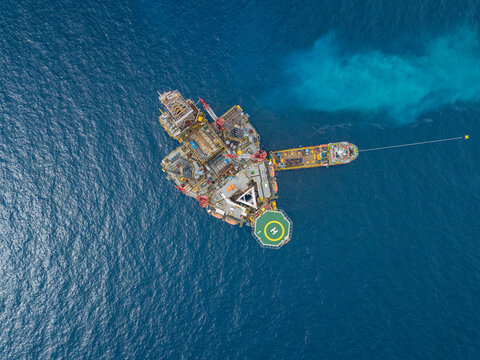
\includegraphics[width=.5\linewidth]{im04}
	\caption{\lr{im04}}
	\label{2}
\end{figure}
 \lr{Active Contours}
  یک روش تقسیم‌بندی است که برای جدا کردن پیکسل‌های مورد نظر از یک تصویر برای پردازش و تحلیل بیشتر استفاده می‌کند.
  \\
کانتورها مرزهایی هستند که ناحیه مورد نظر را در یک تصویر مشخص می‌کنند. هر کانتور از اتصال چندین گره تشکیل شده است.(شکل 
\ref{2}
) در هر مرحله‌ از این الگوریتم سعی می‌کنیم این نقاط را به نحوی تغییر دهیم که در نهایت بر روی حاشیه‌ی جسم قرار گیرند. 
\begin{figure}[H]
	\centering
	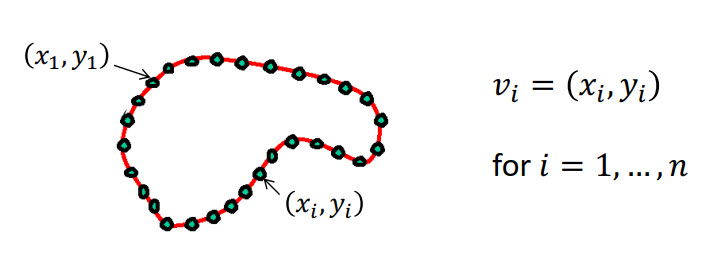
\includegraphics[width=.5\linewidth]{q3-1}
	\caption{\lr{Contour}}
	\label{2}
\end{figure}
این تغییر نقاط به نحوی انجام می‌شود که تابع انرژی زیر کمینه شود. 
\begin{equation*}
	E_{total} = E_{internal} + \gamma\ E_{external}
\end{equation*}
انرژی درونی نماینده شکل کلی کانتور است. انتظار داریم که کانتور ما هموار باشد و یا از شکل هندسی خاصی تبعیت کند. منظور از هموار بودن کانتور این است که نقاط به گونه‌ای نباشند که یکی از نقاط در فاصله دور از توده اصلی نقاط قرار گیرد و یا نقاط از هم فاصله‌های نامتقارن بگیرند. انرژی درونی را با رابطه زیر پیاده سازی کنید:
\begin{equation*}
E_{internal}=\sum_{i=1}^{n}\left(\left(x_{i+1}-x_i\right)^2+\left(y_{i+1}-y_i\right)^2-\alpha\bar{d}\right)^2
\end{equation*}
در رابطه بالا، $ \bar{d} $ میانگین فواصل نقاط در ایتریشن فعلی است. اگر این ترم وجود نداشت کانتور همواره به سمت کوچک شدن پیش میرفت و در نهایت در یک نقطه همگرا میشود. این مورد در شکل 
\ref{3}
نشان داده شده‌است.
\begin{figure}[H]
	\centering
	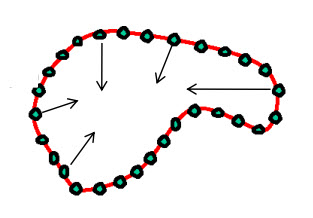
\includegraphics[width=.25\linewidth]{q3-2}
	\caption{}
	\label{3}
\end{figure}
انرژی خارجی مشخص‌کننده‌ی میزان مطابقت کانتور با داده‌های تصویر است و باعث می‌شود که کانتور بر روی حاشیه جسم فیت شود. برای این منظور از جمع مقادیر
 \textbf{منفی اندازه گرادیان} 
در نقاط کانتور صورت می‌پذیرد. (شکل 
\ref{4})
\begin{equation*}
	E_{external}= - \sum_{i=1}^{n} (G_{x}(x_{i},y_{i})^{2} + G_{y}(x_{i},y_{i})^{2})
\end{equation*}
در گرادیان تصویر، حاشیه جسم مقادیر بزرگی دارد و در صورتی که منفی آن مقادیر را در تابع هزینه در نظر بگیریم، مقدار کمینه معادل با قرار گرفتن این نقاط بر روی حاشیه جسم به صورت هموار است. 
\begin{figure}[H]
	\centering
	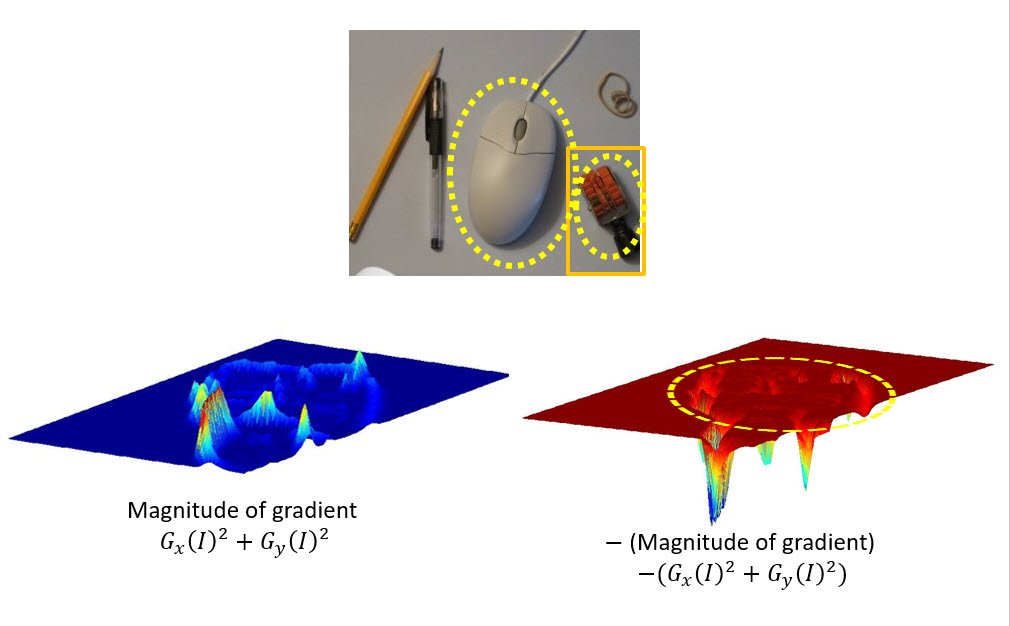
\includegraphics[width=.6\linewidth]{q3-3}
	\caption{}
	\label{4}
\end{figure}
با مشخص شدن تابع هزینه، باید همه نقاط را به گونه‌ای تغییر دهیم که در راستای بیشترین کاهش تابع هزینه حرکت کنیم.  نتیجه مطلوب با استفاده از
\lr{Dynamic Programming}
قابل حصول است. 
در هر 
\lr{iteration}،
 هر کدام از گره‌های کانتور به همسایگی 
$ (n \times n) $
خود (که معمولا
 $ (3 \times 3) $،
 $ (5 \times 5) $
 و یا 
 $ (7 \times 7) $
 است.) بروند و $ E_{total} $ را مینیمم سازند. از آن جایی که هر گره در یک همسایگی خود میتواند حرکت کند، خوش‌بین داریم که با اجرای الگوریتم کانتور به جسم مورد نظر ما نزدیک و نزدیک‌تر شود و به مینیمم تابع هزینه برسد و در مینیمم‌های موضعی گیر نیوفتد. 
 \\
\lr{Dynamic Programming}
روشی است که برای حل این مسئله با هزینه کم محاسباتی. برای یادگیری این الگوریتم از این 
\href{URL}{لینک}
می‌توانید استفاده کنید. 
شرط پایان الگوریتم را رد شدن از حداکثر تعداد ایتریشن و یا حرکت نکردن بیش از $ 90 $ درصد گره‌های کانتور در نظر بگیرید. در صورتی که نیاز به اضافه کردن ترم جدیدی در تابع هزینه دارید، می‌توانید این کار را انجام دهید. در نهایت از شما انتظار می‌رود فیلمی از حرکت گره‌های کانتور از ایتریشن اول تا ایتریشن آخر ارائه دهید. الگوریتم خود را کاملا در گزارش توضیح دهید و پارامتر‌های آزاد مسئله‌ای که انتخاب کرده‌اید را در گزارش ذکر کند.
\\
در زیر پیشنهاد‌هایی جهت پیاده سازی راحت تر شما ارائه می‌شود:
\begin{itemize}
	\item 
$ 20 $ نقطه اولیه را به صورت دستی در کد مشخص کنید. راه دیگر استفاده  از تابع
 \lr{cv2.setMouseCallback}
در پایتون است. با کلیک روی تصویر، چهار نقطه گوشه را بگیرید و سپس $ 20 $ نقطه را به صورت متقارن با استفاده از $ 4 $ نقطه گوشه گرفته شده از کاربر، توزیع کنید و به عنوان نقطه شروع کانتور در نظر بگیرید. شکل 
\ref{5}
را مشاهده کنید. نقاط قرمز گره‌های انتخاب‌شده اولیه است و نقاط سبز به صورت یکنواخت بین این نقاط توزیع شده‌است. 
\begin{figure}[H]
	\centering
	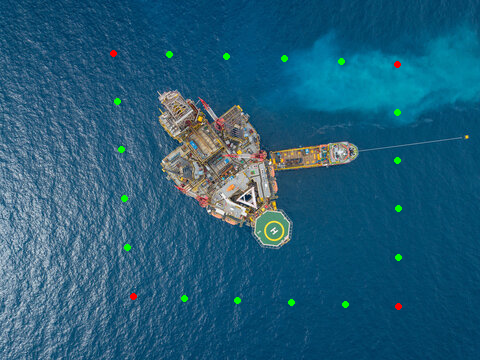
\includegraphics[width=.6\linewidth]{q3-4}
	\caption{}
	\label{5}
\end{figure}
\item
در پایان هر ایتریشن عکس همراه با نقاط کانتور روی آن را در پوشه‌ای به ترتیب ذخیره کنید و در نهایت با استفاده از پکیج
 \lr{ffmpeg} 
 با دستوری مشابه دستور زیر آن ها را به یک فیلم تبدیل کنید (دقت کنید که این پکیج باید بر روی سیستم عامل نصب شود.)
\begin{latin}\small
	\begin{lstlisting}
os.system('ffmpeg -start_number 0 -i Images/%d.png -r 30 -vcodec mpeg4 Contour.MP4');
	\end{lstlisting}
\end{latin} 
\item
پیش پردازش تصویر می‌تواند موثر واقع شود. 
\end{itemize}
نتیجه نهایی را به شکل 
\lr{res13-contour.mp4}
ذخیره نمایید. 
\section{\lr{SLIC Suprepixel}}
\textbf{طراح :‌ امیررضا حاتمی‌پور}
\vspace{0.5cm}
\\
الگوریتم‌های
 \lr{superpixel}، 
گروهی از پیکسل‌ها را که از نظر ساختاری شبیه هم می‌باشند در یک دسته/کلاس قرار می‌دهد. بخاطر بار محاسباتی پایینی که این الگوریتم‌ها دارا می‌باشد، در کاربردهایی مانند تشخیص عمق، تشخیص شی و ... استفاده می‌شوند. در این سوال به پیاده سازی یک الگوریتم ساده 
 به نام
 \lr{Simple Linear Iterative Clustering (SLIC)}
 
 می‌پردازیم.
 (
 \href{http://infoscience.epfl.ch/record/177415/files/Superpixel_PAMI2011-2.pdf}{لینک مقاله مربوطه}
 )
\\
این الگوریتم تصویر را به $ K $ قسمت تقسیم می‌کند. هر پیکسل در فضای پنج بعدی ویژگی‌های رنگ و مختصات به صورت
 \lr{(l,a,b,x,y)}
مشخص مشود. 
می‌توانید بجای فضای رنگ
 \lr{Lab}
  از فضا های دیگر رنگی مانند
  \lr{rgb} 
    یا
  \lr{Hsv}
    و ... استفاده کنید. همچنین تعریف‌های مختلفی برای فاصله مثل نرم یک، نرم دو و... را می‌توانید استفاده کنید. مقدار $ K $  را مقادیر 
    $ 64 $, $ 256 $, $ 1024 $, $ 2048 $
 قرار دهید. 
\begin{enumerate}
	\item 
	تصویر 
	\lr{im05.png}
	را در نظر بگیرید. 
$ K $
مرکز به صورت  یکنواخت در تصویر قرار دهید. (مثلا تصویر را به $ K $ بخش مستطیلی مساوی تقسیم کنید و مرکز هر دسته را وسط مستطیل قرار دهید.)  سپس در یک همسایگی (مثلا $ 5 \times 5 $) در هر مرکز، پیکسلی را که کمترین گرادیان را دارد بعنوان مرکز جدید انتخاب می‌کنیم (برای آن که مراکز انتخاب‌شده در مرزهای تصویر نباشند). 
\item
هر پیکسل را با مراکزی که به فاصله حداکثر 
$ 2S $ 
از آن هستند مقایسه کنید و آن‌ را به بهترین مرکز وصل کنید. مقدار S را میتوانید برابر 
$ \sqrt{N/K} $
بگیرید که N تعداد پیکسل‌های تصویر است. میزان بهینه بودن هر مرکز را از تابع هزینه‌ی زیر متوجه شوید. 
\begin{gather*}
	d_{lab} = \sqrt{(l_{k} -l_{i})^{2} +(a_{k} - a_{i})^{2} +(b_{k} -b_{i})^{2}}
	\\
	d_{xy} = \sqrt{(x_{k} - x_{i})^{2} +(y_{k} - y_{i})^{2}}
	\\
	D = d_{lab} +\alpha d_{xy}
\end{gather*}
که در این تعریف $ i $ اندیس پیکسل‌ $ i $ام است و $ k $ اندیس مرکزی مورد بررسی است. هر پیکسل به دسته‌ای تعلق دارد که فاصله کمتری داشته باشد. پس در پایان این مرحله باید هر پیکسل به یک مرکز مربوط شده باشد. تصویری به اندازه‌ی تصویر اصلی تشکیل دهید که مقدار هر پیکسل برابر با شماره دسته آن پیکسل باشد. چهار نتیجه به دست
آمده برای مقادیر مختلف $ K $
 را به ترتیب
\lr{res14-labels.jpg}،
\lr{res15-labels.jpg}،
\lr{res16-labels.jpg}،
\lr{res17-labels.jpg}
بنامید و ذخیره کنید. 
\item
مرز قطعه‌ها را روی تصویر بکشید و چهار نتیجه به دست آمده برای مقادیر مختلف $ K $  را به ترتیب
\lr{res18-clusters.jpg}،
\lr{res19-clusters.jpg}،
\lr{res20-clusters.jpg}،
\lr{res21-clusters.jpg}
بنامید و ذخیره کنید. در صورت نیاز، با استفاده از فیلتر 
\lr{median}
روی لیبل‌ها، قطعات نهایی را هموار و پیوسته کنید.
\item
تصویری به اندازه تصویر اصلی در تشکیل دهید که مقدار هر پیکسل برابر میانگین مقدار پیکسل‌های داخل قطعه‌ مخصوص‌اش است. چهار نتیجه به دست آمده برای مقادیر مختلف $ K $  را به ترتیب
\lr{res22-Superpixel.jpg}،
\lr{res23-Superpixel.jpg}،
\lr{res24-Superpixel.jpg}،
\lr{res25-Superpixel.jpg}
بنامید و ذخیره کنید.
\end{enumerate}

\section{\lr{   Texture transfer
}}
\textbf{طراح :‌ سیدسعید رضوی}
\vspace{0.5cm}
\\
در این سوال می خواهیم
\lr{pattern}، 
( طرح) یک تصویر را بر روی  یک تصویر دیگر اعمال کنیم . برای مثال به دو شکل پایین و نتیجه حاصل نگاه کنید : 
\begin{figure}[H]
	\centering
	\includegraphics[width=.6\linewidth]{q5-1}
	\caption{}
	\label{6}
\end{figure}
برای اینکار ابتدا لازم است تا تعریف و توضیح مختصری نسبت به 
\lr{texture synthesis}، 
داشته باشیم : 
\\
فرض کنید یک طرح کوچک در اختیار داریم و میخواهیم با استفاده از آن یک تصویر بزرگتر بسازیم (نمونه این کار را میتوانید در تصاویر پایین ببینید ) 

\begin{figure}[H]
	\centering
	\includegraphics[width=.6\linewidth]{q5-2}
	\caption{}
	\label{7}
\end{figure}
برای ساختن تصویر بزرگتر روش های متفاوتی در پیش رو داریم: 


\begin{enumerate}
	\item 
	اگر بدون هیچ زحمتی هر بار بخشی از طرح اولیه را به صورت بلاک هایی در کنار هم قرار دهیم به تصویر زیر میرسیم: 
	\begin{figure}[H]
		\centering
		\includegraphics[width=.6\linewidth]{q5-3}
		\caption{}
		\label{8}
	\end{figure}
	\item
	راه دیگری که در پیش داریم این است که اولین بلوک
	\lr{(block)}، 
	 انتخاب شده به صورت رندوم و کاملا دلخواه  باشد اما بقیه بلوک ها را متناسب با ناحیه اورلپ انتخاب کنیم . به این صورت ناحیه ای را به عنوان اورلپ در نظر بگیریم  و آن ناحیه اورلپ را در عکس
	 \lr{(texture )}، 
	 خود سرچ کنیم و نواحی با کمترین هزینه یا بیشترین شباهت ( هزینه را میتوان به گونه های مختلفی تعریف کرد و یکی از بهترین تعاریف ،
	  \lr{L2 norm}، 
	  میباشد که برابر است با توان 2 اختلاف پیکسل ها در ناحیه اورلپ ) را در نظر گرفته  ، یکی از آنها را  را انتخاب کنیم و به بلوک دوم بچسبانیم  و ادامه تصویر را بسازیم . اگر این کار را بکنیم داریم : 
	  \begin{figure}[H]
	  	\centering
	  	\includegraphics[width=.6\linewidth]{q5-4}
	  	\caption{}
	  	\label{9}
	  \end{figure}
  همانطور که مشاهده میکنید کیفیت ساخت تصویر بسیار بهتر شده اما باز هم ناپیوستگی ها در تصویر حاصل مشخص است . برای رفع این مشکل از روش سوم استفاده میکنیم :
	\item
	می توانیم از روش
	 \lr{ minimum boundary cut}، 
	 که در تمرین سری 5 نیز با آن آشنا شدید استفاده کنید . اگر از این روش استفاده کنیم نتیجه زیر حاصل میشود :  
\begin{figure}[H]
	\centering
	\includegraphics[width=.6\linewidth]{q5-5}
	\caption{}
	\label{10}
\end{figure}
اگر بخواهیم طرح کلی از فرایند
  \lr{texture synthesis},
  داشته باشیم به شکل زیر میرسیم : 
\begin{figure}[H]
	\centering
	\includegraphics[width=.6\linewidth]{q5-6}
	\caption{}
	\label{11}
\end{figure}
	حال توضیح مختصری در رابطه  با
	 \lr{texture transfer}
	 میرسیم : 
	 \\
	 ورودی ما یکی پترن
	 \lr{(texture)}
	 و دیگری تصویر هدف( که میخواهیم پترن مدنظر روی آن اعمال کنیم ) میباشد .   برای این کار علاوه بر اینکه هدف مینیمم کردن هزینه در ناحیه اورلپ می باشد باید بلوک انتخاب شده در هر مرحله ( به جز مرحله اول که انتخاب بلوک رندوم است ) علاوه بر برآورده کردن شرط کمترین هزینه بین ناحیه اورلپ بلوک جدید و قبلی آن در پترن ورودی ، باید کمترین هزینه را  بین بلوک جدید و متناظر آن در همان مختصات در تصویر هدف برآورده شود. به عبارتی هدف پیدا کردن بلوکی است که شرط زیر را برآورده کند : 
	\\
	$ Minimize  : ɑ[cost_function (blocki and blocki-1 in  texture image)+(1-ɑ)cost_function(blocki in texture image and it’s correspondence in target image)]$
	برای مطالعه بیشتر مقاله را از
	 (
	\href{https://people.eecs.berkeley.edu/~efros/research/quilting/quilting.pdf}{این لینک}
	) مشاهده کنید  .
	\\
	حال که با 
	\lr{texture transfer}
	آشنا شدید همین الگوریتم را برای دو تصویر که در فایل زیپ با نام های 
	\lr{im06.jpg}
	و
	\lr{im07.jpg}
	قرار دارند انجام دهید و نتیجه نهایی را با نام
	\lr{res26-texture.jpg}
	ذخیره نمایید . 
	
\end{enumerate}

\end{document}